

\chapter{Cadre général du projet}

\newpage
%Intro\footnotemark\\
%note en bas de page

\textbf{\huge Introduction} \\[1cm]



%inclusion d'une mage dans le document
%\begin{figure}[!h]
%\begin{center}
%taille de l'image en largeur
%remplacer "width" par "height" pour régler la hauteur
%\includegraphics[width=15cm]{presentation/schema}
%\end{center}
%légende de l'image
%\caption{Schéma descriptif}
%\end{figure}

%Contenu de la note précédemment marquée avec \footnotemark
%\footnotetext{Note bas de page "intro"}
\textsf{\fontfamily{qtm}\selectfont\scalefont{1.3}
    Ce chapitre est consacré à la présentation du cadre général de notre projet. En premier lieu, nous présentons la société d’accueil. Par la suite, nous présentons le cadre du projet qui comporte la problématique. On finit par une présentation de la méthodologie que nous allons adopter pour le développement de notre projet.}\\[1cm]

%retour à la ligne (alinea)

%saut de paragraphe

%\newpage

\section{\LARGE Société d’accueil }
\texttt{}\\[0.1cm]
\textsf{\fontfamily{qtm}\selectfont\scalefont{1.3}Dans ce qui suit,nous présentons la société d'accueil ainsi que son domaine d'activié.}
\texttt{}\\[0.1cm] 
\subsection{\Large   Identité }
\texttt{}\\[0.5cm]
\textsf{\fontfamily{qtm}\selectfont\scalefont{1.3} Mobelite est umne agence spécialisée dans le conseil en stratégie mobile, la conception et le développement d’applications mobiles , de sites web et le marketing mobile. Mobelite est forte d’une équipe d’experts dans la réalisation d’applications mobiles sur les platefores les plus répandues et les applications Web. Mobelite dispose d’équipes commerciales et marketing à Paris (France), et d’équipes de développement à Tunis et Monastir (Tunisie).
}
\texttt{}\\[0.1cm]
\begin{figure}[H]
    \begin{center}
    
    \fbox{
\includegraphics[width=10cm]{presentation/logomob.png}}

    \end{center}
    
    \caption{Logo de la société mobelite}
\end{figure}
\newpage
\subsection{\Large Activités de mobelite}
\texttt{}\\[0.5cm]
\textsf{\fontfamily{qtm}\selectfont\scalefont{1.3} Mobelite est une société experte dans que ce création des sites web intuitifs et ergonomiques pour tous les supports soit desktop, tablette ou mobile et avec les plus récente technologies et Framework de développement comme React JS, Node JS et Angular.Les équipes de mobelite maîtrisent parfaitement la conception et le développement d’applications natives iOS et Android pour tous les différents supports que ce soit smartphone, tablette, Watch et TV. Mobelite excelle dans le conseil de ses clients dans différentes parties de projets comme l'analyse des besoins, UX/UI, la conception, le design,le développement, SEO, DevOps et l'hébergement. Tout ça est réalisé selon la méthodologie Agile, afin de maximiser les possibilités d’itérations sur le concept, et d’introduire plus de flexibilité sur les arbitrages fonctionnels à faire.(voir figure 1.2)
}
\texttt{}\\[0.1cm]
\begin{figure}[H]
    \centering
    \fbox{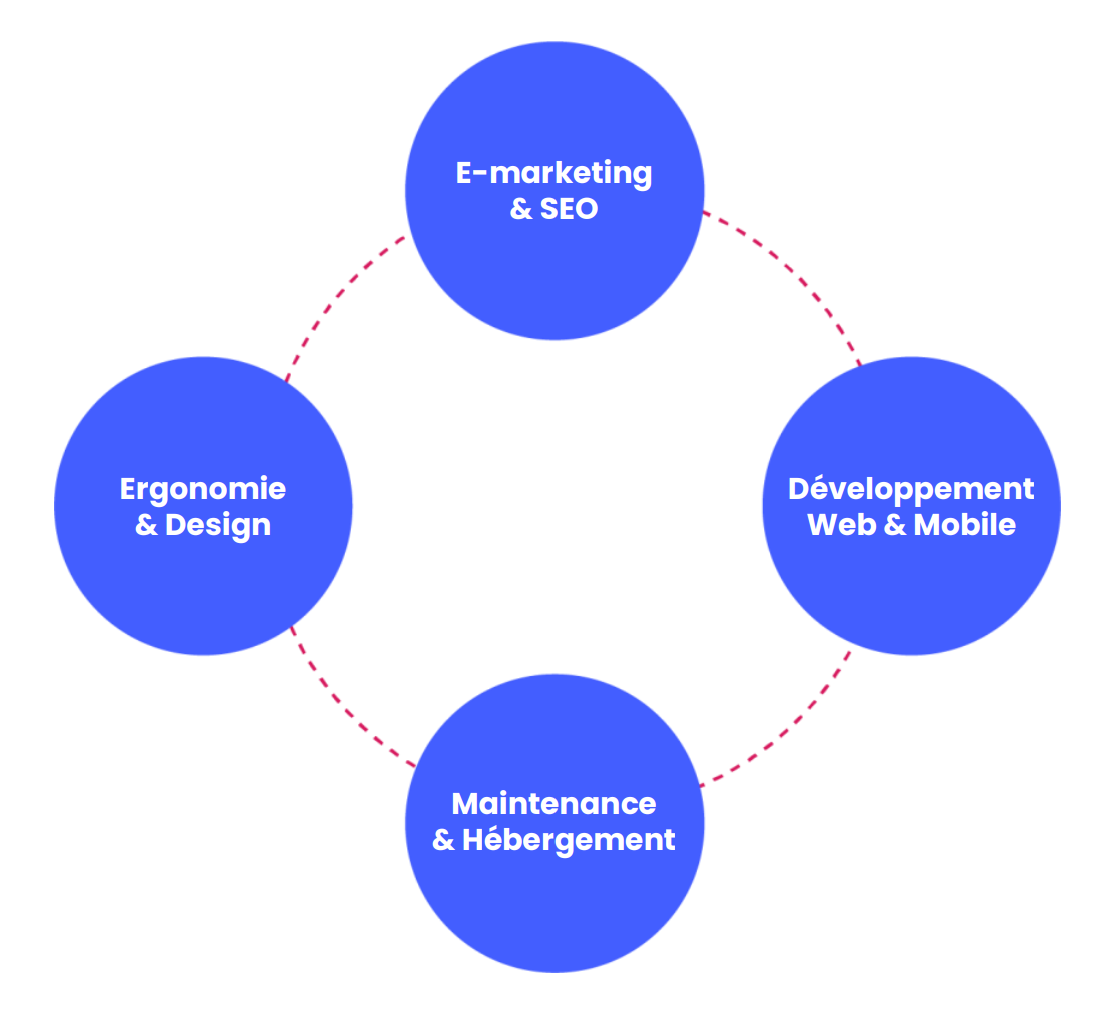
\includegraphics[width=10cm]{presentation/domaine.png}}
    \caption{différents domaines de mobelite}
    \label{fig:Activités de mobilite}
\end{figure}
\newpage
\section{\LARGE Problématique }
\texttt{}
\textsf{\fontfamily{qtm}\selectfont\scalefont{1.3}
    Le déploiement des systèmes de gestion de code source telle que Nexus, SonarQube ou le Monitoring sur un seul serveur local présente plusieurs problèmes qui affectent la performance de serveur et qui rendent l’exécution des diffèrent application ou l’ajout des nouvelles fonctionnalités plus difficile . Aussi, la maintenance de plusieurs applications en même temps sera compliquée et nécessite une planification minutieuse pour éviter l’interruption des processus d’autres applications. Les besoins d’entreprise changent au cours des temps et la capacité d'un seul serveur sera insuffisante pour rependre à la charge des données. Les mise à jour des applications peutent impacter d'autres applications ou seront impossibles à cause de limites des ressources. En terme de sécurité, une attaque sur le serveur cause une perte des données très grand que sera difficile de récupérer en conséquence de l’utilisation d'un seul serveur.
}

\section{\LARGE Notion de base}
\textsf{\fontfamily{qtm}\selectfont\scalefont{1.3}Dans ce qui suit ,nous présentons les notions de base}
\subsection{\LARGE  Microservice}
\textsf{\fontfamily{qtm}\selectfont\scalefont{1.3} Avant l'apparition de l'architecture micro-service, les applications sont construites de
    manière monolithique, qui est considérée aujourd’hui comme méthode impertinente, L’utilisation de l'architecture monolithique, rend l’application très
    volumineuse avec des difficultés à enrichir les fonctions et le traitement des problèmes.
    Les microservices créent une application unique à partir de plusieurs petits services reliés de manière flexible.
    Ces services ont leur propre logique et leur propre base de données pour un usage spécifique. Chaque service peut être développé, mis à jour, déployé et mis à l’échelle sans affecter les autres services. Les mises à jour logicielles peuvent être plus fréquentes, ce qui améliore la fiabilité, la disponibilité et les performances.(Voir figure 1.3)
}
\begin{figure}[H]
    \begin{center}
    \fbox{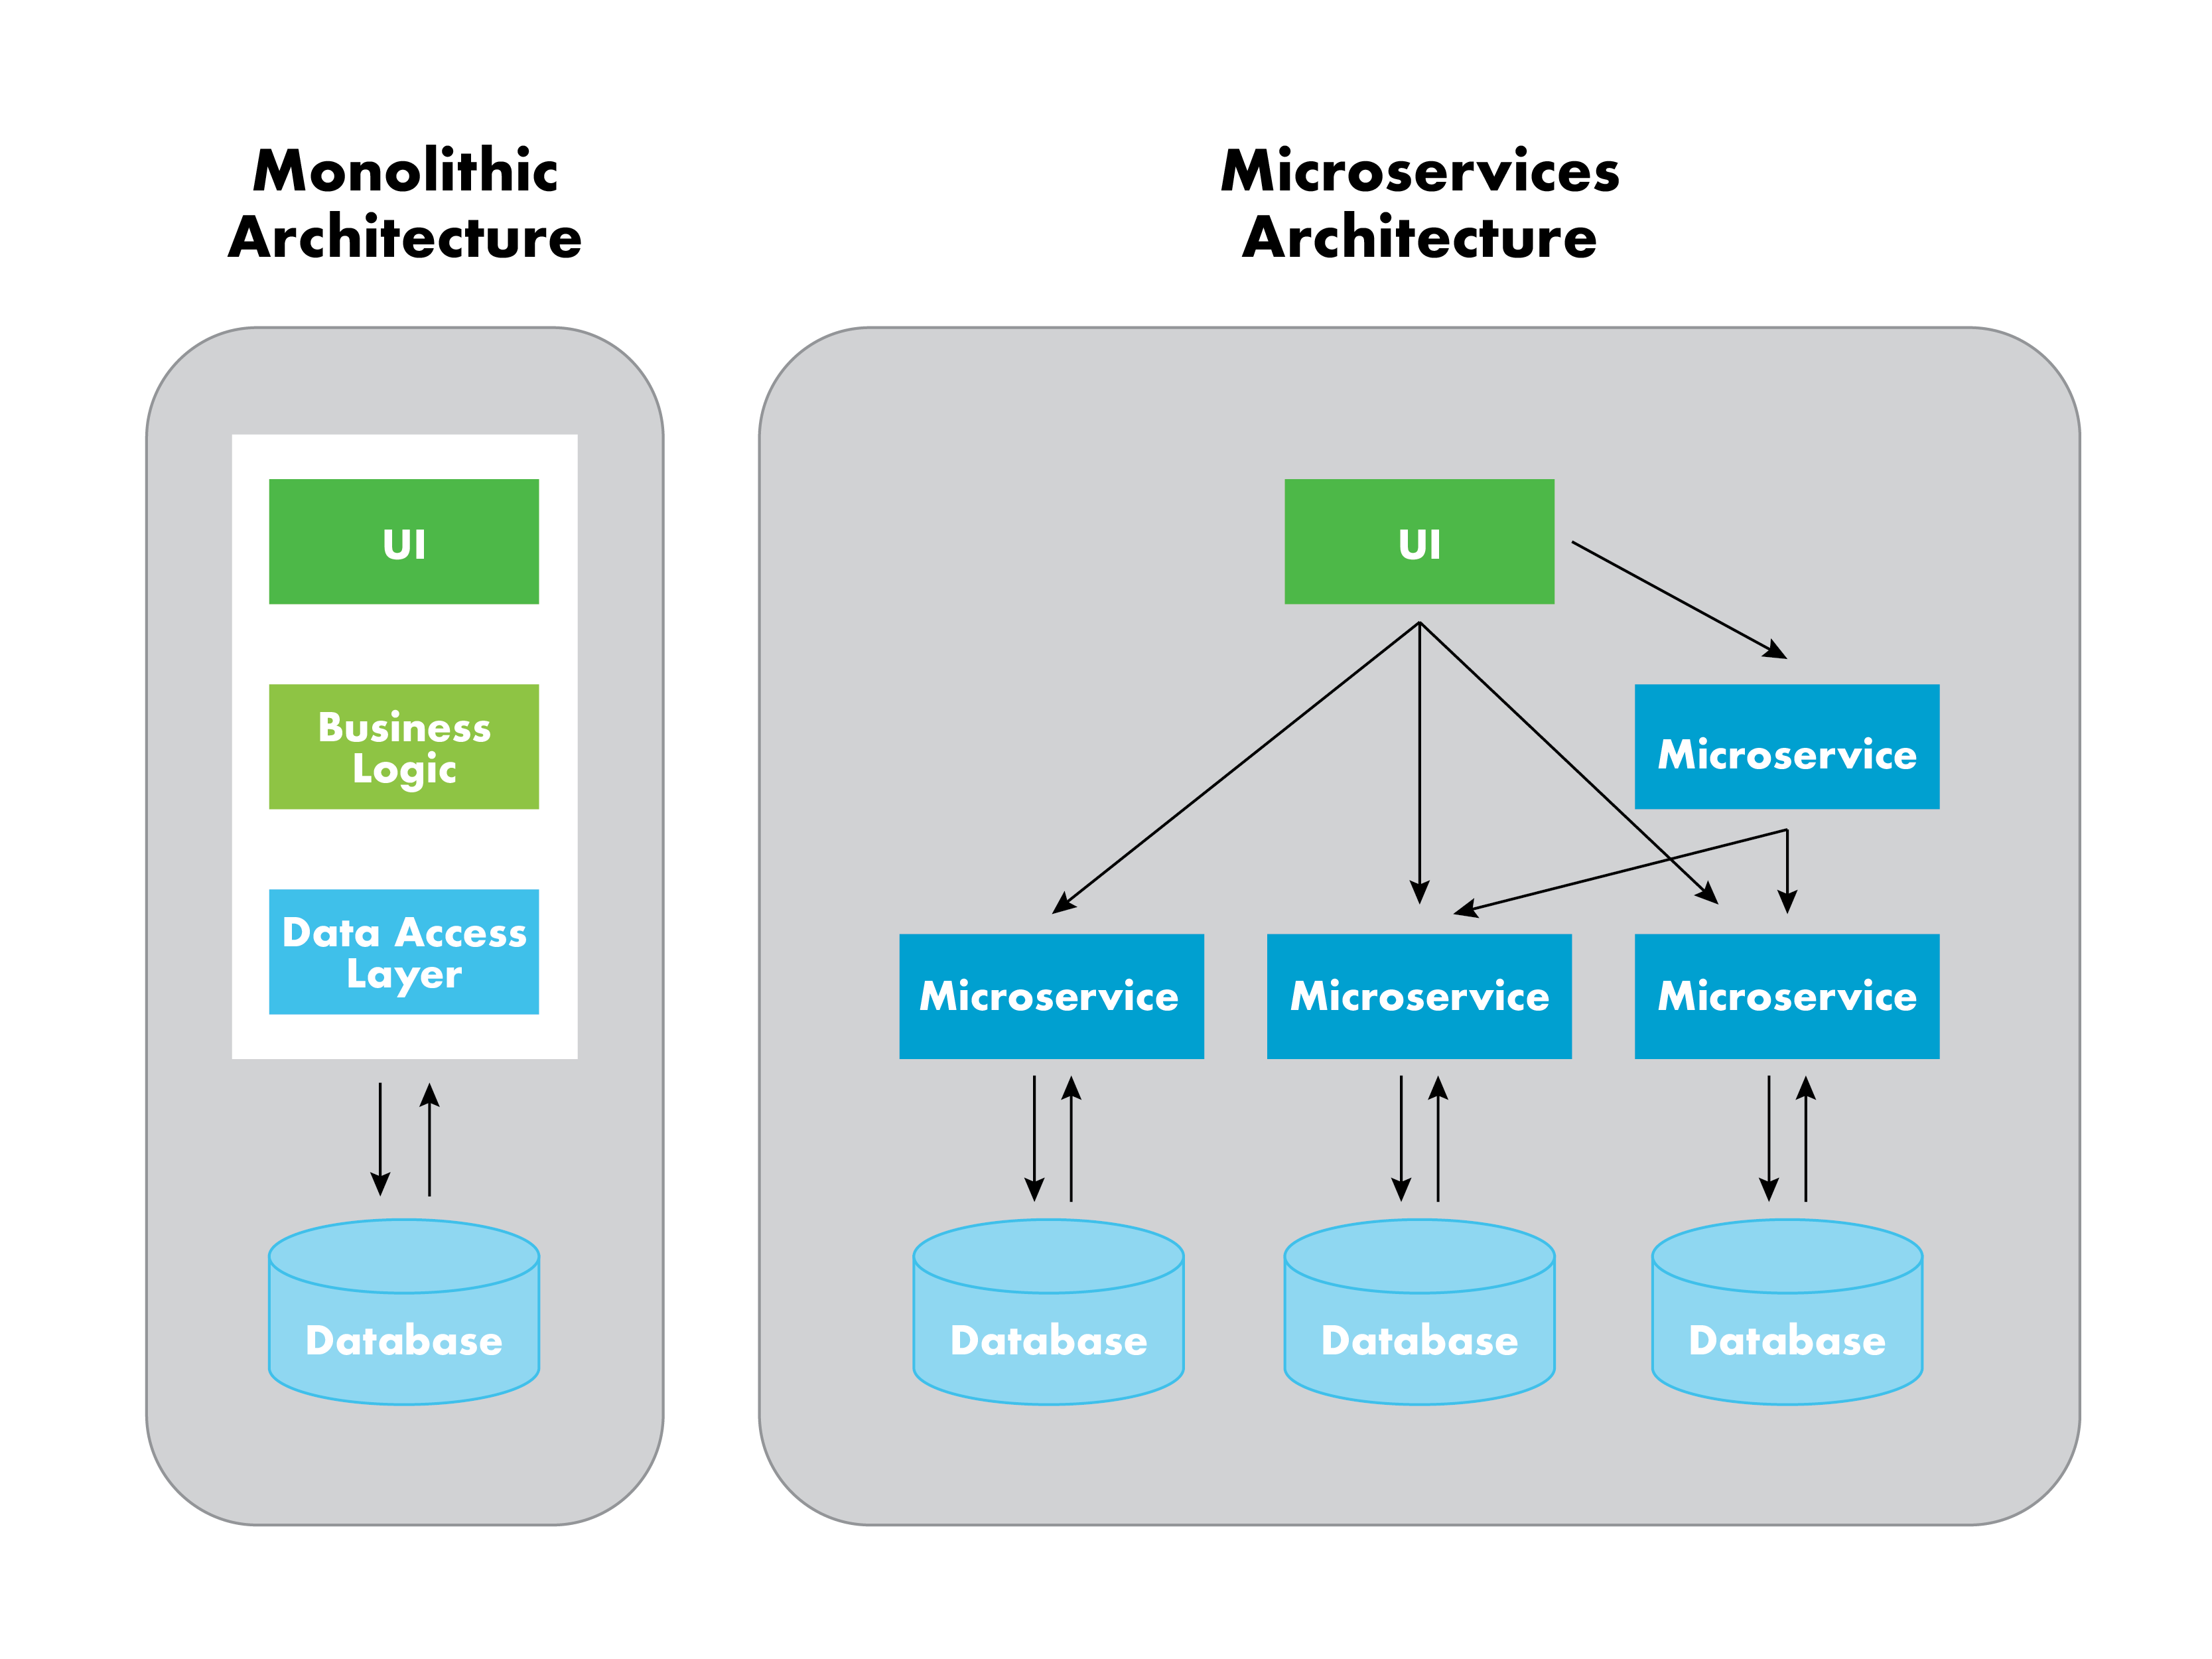
\includegraphics[height=11cm]{presentation/Microservice.png}}
    \end{center}
    \caption{Architecture monolithique vs Micro services}
\end{figure}
\subsection{\Large  Devops}
\texttt{}\\[0.5cm]
\textsf{\fontfamily{qtm}\selectfont\scalefont{1.3} Combinant développement (Dev) et opérations (Ops), DevOps est l'union des personnes, des processus et des technologies destinés à fournir continuellement de la valeur aux clients.
    DevOps permet la coordination et la collaboration des rôles autrefois cloisonnés( développement, opérations informatiques, ingénierie qualité et sécurité) pour créer des produits plus performantes et plus fiables. En adoptant une culture DevOps ,ainsi que des pratiques et outils DevOps, les équipes peuvent mieux répondre aux besoins des clients, accroître la confiance suscitée par les applications qu'elles développent, et atteindre plus rapidement les objectifs de leur entreprise.\cite{1}(voir figure 1.3)}
    \begin{figure}[H]
    \begin{center}

    \fbox{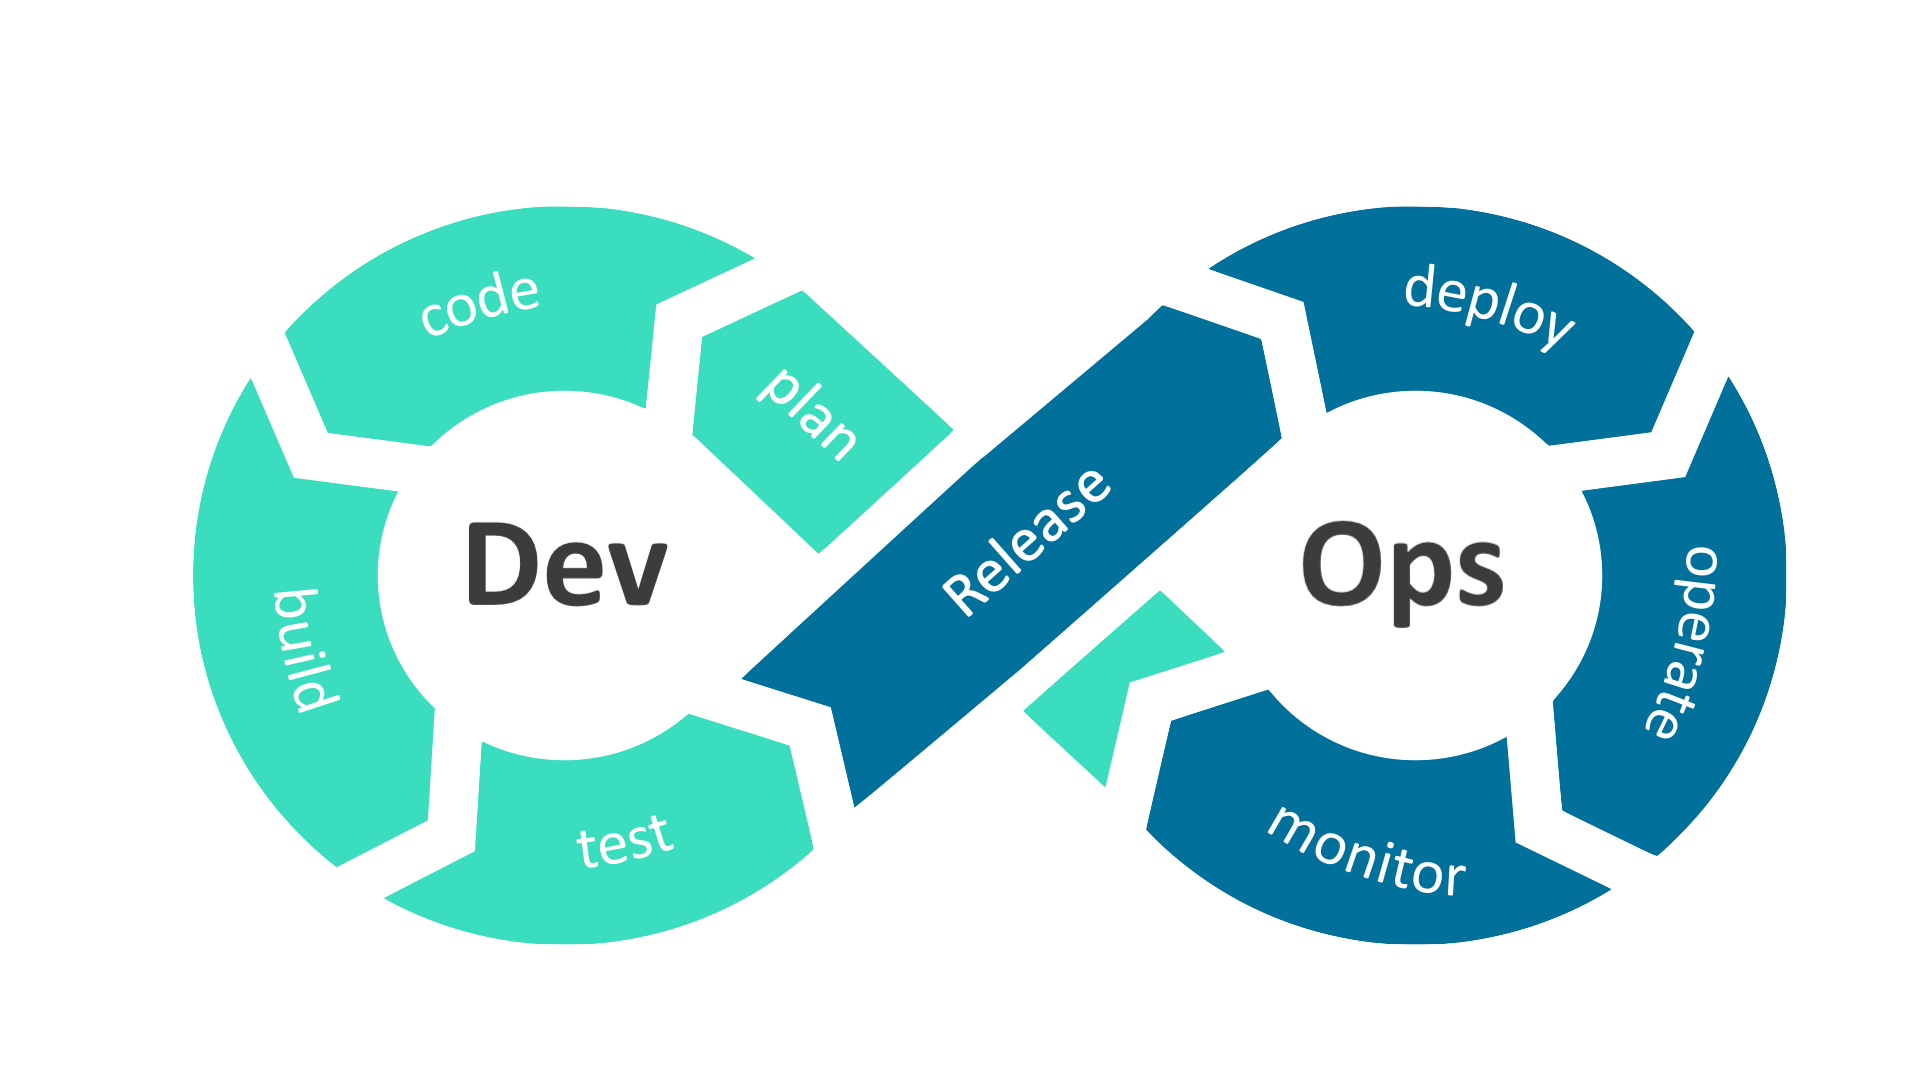
\includegraphics[height=8cm]{presentation/devops.png}}
    \end{center}

    \caption{Cycle de vie DevOps}
\end{figure}
\texttt{}\\[0.1cm]
\subsection{\Large  Cloud}
\texttt{}\\[0.1cm]
\textsf{\fontfamily{qtm}\selectfont\scalefont{1.3} Le cloud n’est pas une entité physique, mais un vaste réseau de serveurs distants éparpillés tout autour de la planète, reliés entre eux, et destinés à fonctionner comme un écosystème unique. Ces serveurs sont conçus pour stocker et gérer des données, exécuter des applications, ou fournir du contenu ou des services (vidéos diffusées en continu, courrier web, logiciels bureautiques de productivité et autres réseaux sociaux). Au lieu d’accéder à des fichiers et données stockées sur un ordinateur local ou personnel, vous accédez à ces ressources en ligne à partir de n’importe quel appareil compatible avec Internet : les informations sont disponibles en tout lieu et tout le temps.\cite{2} }
\subsubsection{\Large Modèles de services }
\texttt{}\\[0.1cm]
\textsf{\fontfamily{qtm}\selectfont\scalefont{1.3}Il existe 3 modèles de services:}
\texttt{}\\[0.1cm]
\par \noindent \textbf{\LARGE - Software as a Service (SaaS) : }\textsf{\fontfamily{qtm}\selectfont\scalefont{1.3} Le Software as a Service, également connu sous le nom de SaaS, est un service basé sur le cloud où, au lieu de télécharger un logiciel que votre PC de bureau ou votre réseau professionnel peut exécuter et mettre à jour, vous accédez à une application via un navigateur internet. L'application logicielle peut être un logiciel de bureautique ou de communication unifiée parmi un large éventail d'autres applications professionnelles disponibles.\cite{3} (voir figure 1.5)}
\begin{figure}[H]
    \begin{center}
\fbox{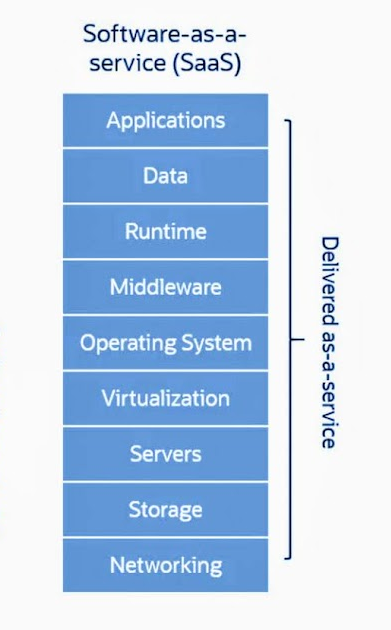
\includegraphics[height=8cm]{presentation/saas.png}}
    \end{center}

    \caption{ Architecture SaaS
    }
\end{figure}
\noindent \textbf{\LARGE - Platform as a Service (PaaS) : }\textsf{\fontfamily{qtm}\selectfont\scalefont{1.3} La Platform-as-a-service (PaaS) est un type d'offre de cloud computing dans lequel un fournisseur de services fournit une plateforme à ses clients, leur permettant de développer, d'exécuter et de gérer des applications commerciales sans avoir à construire et à maintenir l'infrastructure que ces processus de développement de logiciels requièrent généralement.(Voir figure 1.6)\cite{4}}\\[0.1cm]
\begin{figure}[H]
    \begin{center}

    \fbox{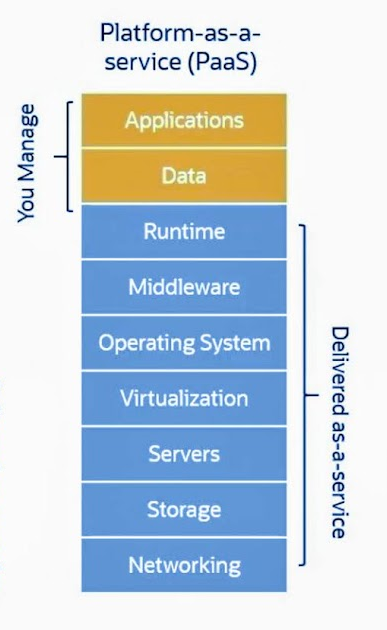
\includegraphics[height=8cm]{presentation/paas.png}}
    \end{center}

    \caption{ Architecture PaaS}
\end{figure}
\noindent \textbf{\LARGE - Infrastructure as a Service (IaaS) : }\textsf{\fontfamily{qtm}\selectfont\scalefont{1.3} Infrastructure as a service (IaaS) est un type de service de cloud computing qui offre des ressources de calcul, de stockage et de mise en réseau essentielles à la demande, et sur une base de paiement à l’utilisation.(Voir figure 1.7)\cite{5}}\\[0.1cm]
\begin{figure}[H]
    \begin{center}

    \fbox{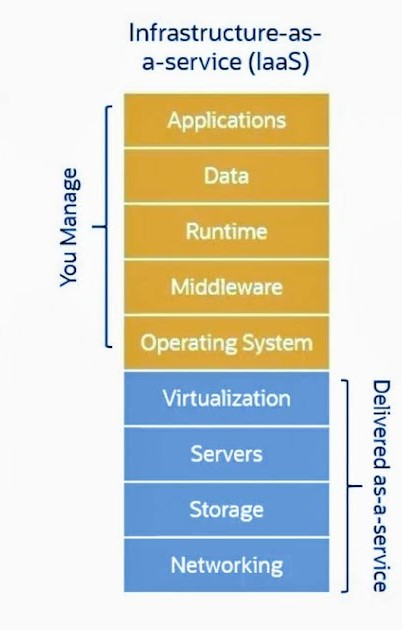
\includegraphics[height=8cm]{presentation/iaas.png}}
    \end{center}

    \caption{ Architecture IaaS}
\end{figure}
\subsubsection{\Large Les modèles de déploiement }
\texttt{}\\[0.1cm]
\textsf{\fontfamily{qtm}\selectfont\scalefont{1.3}Il esxiste 3 modèles de déploiement:}
\texttt{}\\[0.1cm]
\par \noindent \textbf{\LARGE - Cloud Privé :  }\textsf{\fontfamily{qtm}\selectfont\scalefont{1.3} Le cloud privé est un modèle informatique qui offre un environnement propriétaire dédié à une seule entité commerciale. Comme les autres types d'environnements du cloud computing, le cloud privé fournit des ressources informatiques étendues et virtualisées via des composants physiques stockés sur place ou dans le centre de données d'un fournisseur.\cite{6}}\\[0.1cm]

\noindent \textbf{\LARGE - Cloud Public: }\textsf{\fontfamily{qtm}\selectfont\scalefont{1.3} Le cloud public est un type de calcul dans lequel les ressources sont proposées par un fournisseur tiers via Internet, et sont partagées par les organisations et les individus qui souhaitent les utiliser ou les acheter.\cite{7}}\\[0.1cm]

\noindent \textbf{\LARGE - Cloud Hybrid :  }\textsf{\fontfamily{qtm}\selectfont\scalefont{1.3} Un cloud hybride est un environnement informatique mixte dans lequel des applications s'exécutent à l'aide d'une combinaison de ressources de calcul, de stockage et de services dans différents environnements (clouds publics et clouds privés, y compris des centres de données sur site ou en périphérie).\cite{8}}\\[0.1cm]

\section {\Large méthodologie de développement }
\textsf{\fontfamily{qtm}\selectfont\scalefont{1.3}
Avant de mettre en oeuvre un projet informatique, il est nécessaire de choisir une méthodologie de travail et un processus de suivi pour aboutir à un logiciel fiable.
C’est un cadre utilisé pour structurer, planifier et contrôler le développement d’une application.
Il existe une diversité de méthodologies disponibles et
chacune offre des avantages donc choisir une n’est pas une tâche facile.
Pour ça nous procéderons à une étude à propos les méthodes existantes.}\\[0.2cm]
\subsection{\Large Méthode   classique}
\texttt{}\\[0.1cm]
\textsf{\fontfamily{qtm}\selectfont\scalefont{1.3}
 la méthode classique de gestion de projet est une méthode qui suit un processus strict et séquentiel, où chaque étape du projet doit être terminée avant de passer à la suivante. Le projet est cadré et planifié en amont, en fonction des besoins du client définis dans un cahier des charges. Le client n’intervient pas en cours de projet et le contrôle qualité a lieu à la fin. Il existe plusieurs méthodes classiques, comme la méthode Waterfall (en cascade) ou le Cycle en V.Comme ce suit l'exemple du processus de méthode en V (Voir figure 1.8)}.\\[0.1cm]
\texttt{}
\begin{figure}[H]
    \begin{center}
    
        \fbox{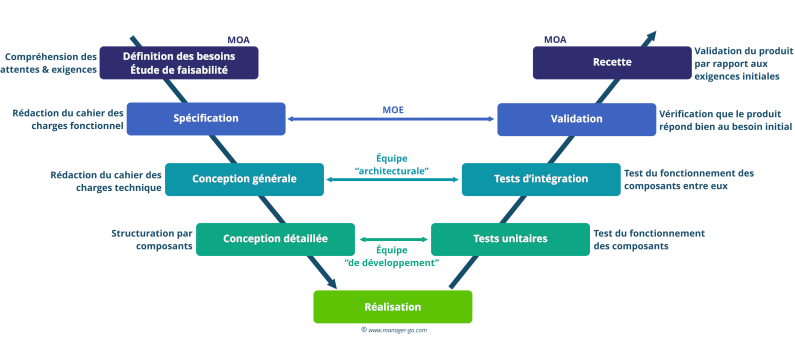
\includegraphics[height=7cm]{Cycle-V-min}}
    \end{center}
    \caption{Processus de méthode cycle en V}
\end{figure}
\subsection{\Large Méthode  du processus unifié }
\texttt{}\\[0.2cm]
\textsf{\fontfamily{qtm}\selectfont\scalefont{1.3}
En résumé, la méthode du processus unifié est une méthode de développement de logiciel orientée objet qui se base sur des principes.
Une approche basée sur les modèles, et en particulier les modèles UML, qui permettent de représenter graphiquement les différents aspects du système.
Une approche itérative et incrémentale, qui divise le projet en plusieurs cycles de développement composés de quatre phases : inception, élaboration, construction et transition. Chaque cycle produit une version du système qui réduit les incertitudes et les risques (voir figure 1.9). 
}

\begin{figure}[H]
    \begin{center}
        %taille de l'image en largeur
        %remplacer "width" par "height" pour régler la hauteur
    \fbox{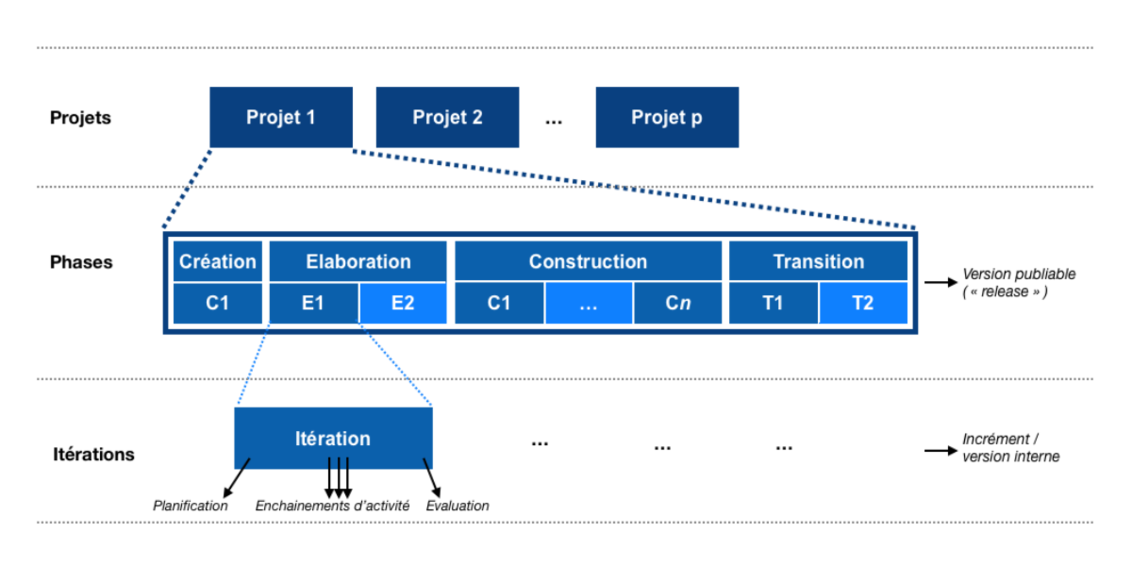
\includegraphics[height=6cm]{2 tracks unified process}}
    \end{center}
    %légende de l'image
    \caption{Cycle de vie de projet avec le processus unifié }
\end{figure}
\texttt{}\\[0.2cm]
\subsection{\Large Méthode agile }
\texttt{}\\[0.1cm]
\textsf{\fontfamily{qtm}\selectfont\scalefont{1.3} la méthode agile est une façon de travailler en équipe qui favorise la collaboration, la flexibilité et la livraison rapide de valeur aux clients. Au lieu de suivre un plan rigide et détaillé, les équipes agiles s’adaptent aux besoins et aux changements tout au long du projet. Elles découpent le travail en petites tâches appelées “user stories” et les réalisent lors de cycles courts appelés “sprints”. Elles communiquent régulièrement entre elles et avec le client pour s’assurer de la qualité et de la satisfaction. Il existe plusieurs méthodes agiles, comme Scrum, Kanban ou XP, qui proposent des règles et des pratiques spécifiques pour mettre en oeuvre cette philosophie.
}\\[0.2cm]

\subsubsection{\Large    Présentation de la méthodologie Scrum}
\texttt{}\\[0.1cm]
\textsf{\fontfamily{qtm}\selectfont\scalefont{1.3}
Scrum est une méthodologie agile pour l'élaboration, la réalisation et le soutien de projets complexes. Elle est basée sur la division du produit sur différentes itération sprints.
Scrum est plus utile lorsque les exigenes sont variables et peuvent changer beaucoup de fois au cours du cycle de vie, ce qui donne donc la capacité d'avoir un projet flexible capable de traiter les changements fréquents.}\\[0.2cm]
\subsubsection{\Large    Acteurs de la méthode agile Scrum}
\texttt{}\\[0.1cm]
\textsf{\fontfamily{qtm}\selectfont\scalefont{1.3}
Méthode agile Scrum se compose par 3  acteurs ce suit : }\\[0.1cm]
\par \noindent \textbf{\LARGE - Scrum Master : }\textsf{\fontfamily{qtm}\selectfont\scalefont{1.3} Il s'agit de la personne chargée d'orienter l'équipe de travail vers la bonne voie, d'assurer la bonne pratique des règles de la méthode Scrum et d'organiser son équipe.} \\[0.1cm]

\noindent \textbf{\LARGE - Product Owner : }\textsf{\fontfamily{qtm}\selectfont\scalefont{1.3} il représente les clients et assure que leurs besoins et visions soient réalisés dans le projet, il travaille généralement en collaboration directe avec l’équipe de développement. }\\[0.1cm]

\noindent \textbf{\LARGE - Equipe de développement : }\textsf{\fontfamily{qtm}\selectfont\scalefont{1.3}sont les personnes responsables de la transformation des besoins du client. Ces besoins sont définis par le Product Owner à travers des fonctions utilisables. L'équipe est composée d'au moins 3 personnes jouant les rôles de développeur ou de concepteur.}\\[0.1cm]
\subsubsection{\Large Évènements de la méthode agile Scrum }
\texttt{}\\[0.1cm]
\textsf{\fontfamily{qtm}\selectfont\scalefont{1.3} Scrum définit cinq types d'évènements :}\\[0.1cm]
\par \noindent \textbf{\LARGE - Le sprint :}\textsf{\fontfamily{qtm}\selectfont\scalefont{1.3} chaque sprint est de durée maximale de 4 semaines pendant laquelle une version de produit est réalisée. Un sprint terminé un nouveau a déjà commencé avec une liste de fonctionnalités et un objéctif à réaliser.} \\[0.1cm]

\noindent \textbf{\LARGE - Planification d’un sprint : }\textsf{\fontfamily{qtm}\selectfont\scalefont{1.3} À chaque début de sprint, cette réunion est conçue pour déterminer les tâches à réaliser pendant le sprint. L’organisation de ces tâches est effectuée par l’équipe de développement et le Product Owner. }\\[0.1cm]

\noindent \textbf{\LARGE - Mêlée quotidienne : }\textsf{\fontfamily{qtm}\selectfont\scalefont{1.3} C'est une réunion d'une durée de 15 minutes faite par l’équipe chaque jour pour définir l’objectif de la journée et identifier les obstacles s’il y en a quelques-uns.}\\[0.1cm]

\noindent \textbf{\LARGE - Revue de sprint : } \textsf{\fontfamily{qtm}\selectfont\scalefont{1.3} Représente le travail réalisé par l’équipe au cours du sprint et le comparer avec le produit attendu.}\\[0.1cm]

\noindent \textbf{\LARGE - Rétrospective de sprint : }\textsf{\fontfamily{qtm}\selectfont\scalefont{1.3} Le but de cet événement est de déterminer les problèmes intervenus dans la période du sprint, l’efficacité des outils et déterminer ce qui peut être amélioré.}\\[0.1cm]

\subsubsection{ \Large Les artefacts}
\texttt{}\\[0.1cm]
\noindent \textbf{\LARGE - Product Backlog : }\textsf{
    \fontfamily{qtm}\selectfont\scalefont{1.3} Il s’agit d’une liste des besoins et exigences à recueillir pour créer le produit désiré, ce document est la responsabilité de Product Owner.(voir figure 1.8)}\\[0.1cm]

\noindent \textbf{\LARGE - Sprint Backlog : }\textsf{\fontfamily{qtm}\selectfont\scalefont{1.3} c’est l’ensemble des données permettant la réalisation les objectifs du sprint. Ce document est mis à jour par l’équipe de développement régulièrement.}
\texttt{}
\begin{figure}[H]
    \begin{center}
        %taille de l'image en largeur
        %remplacer "width" par "height" pour régler la hauteur
    \fbox{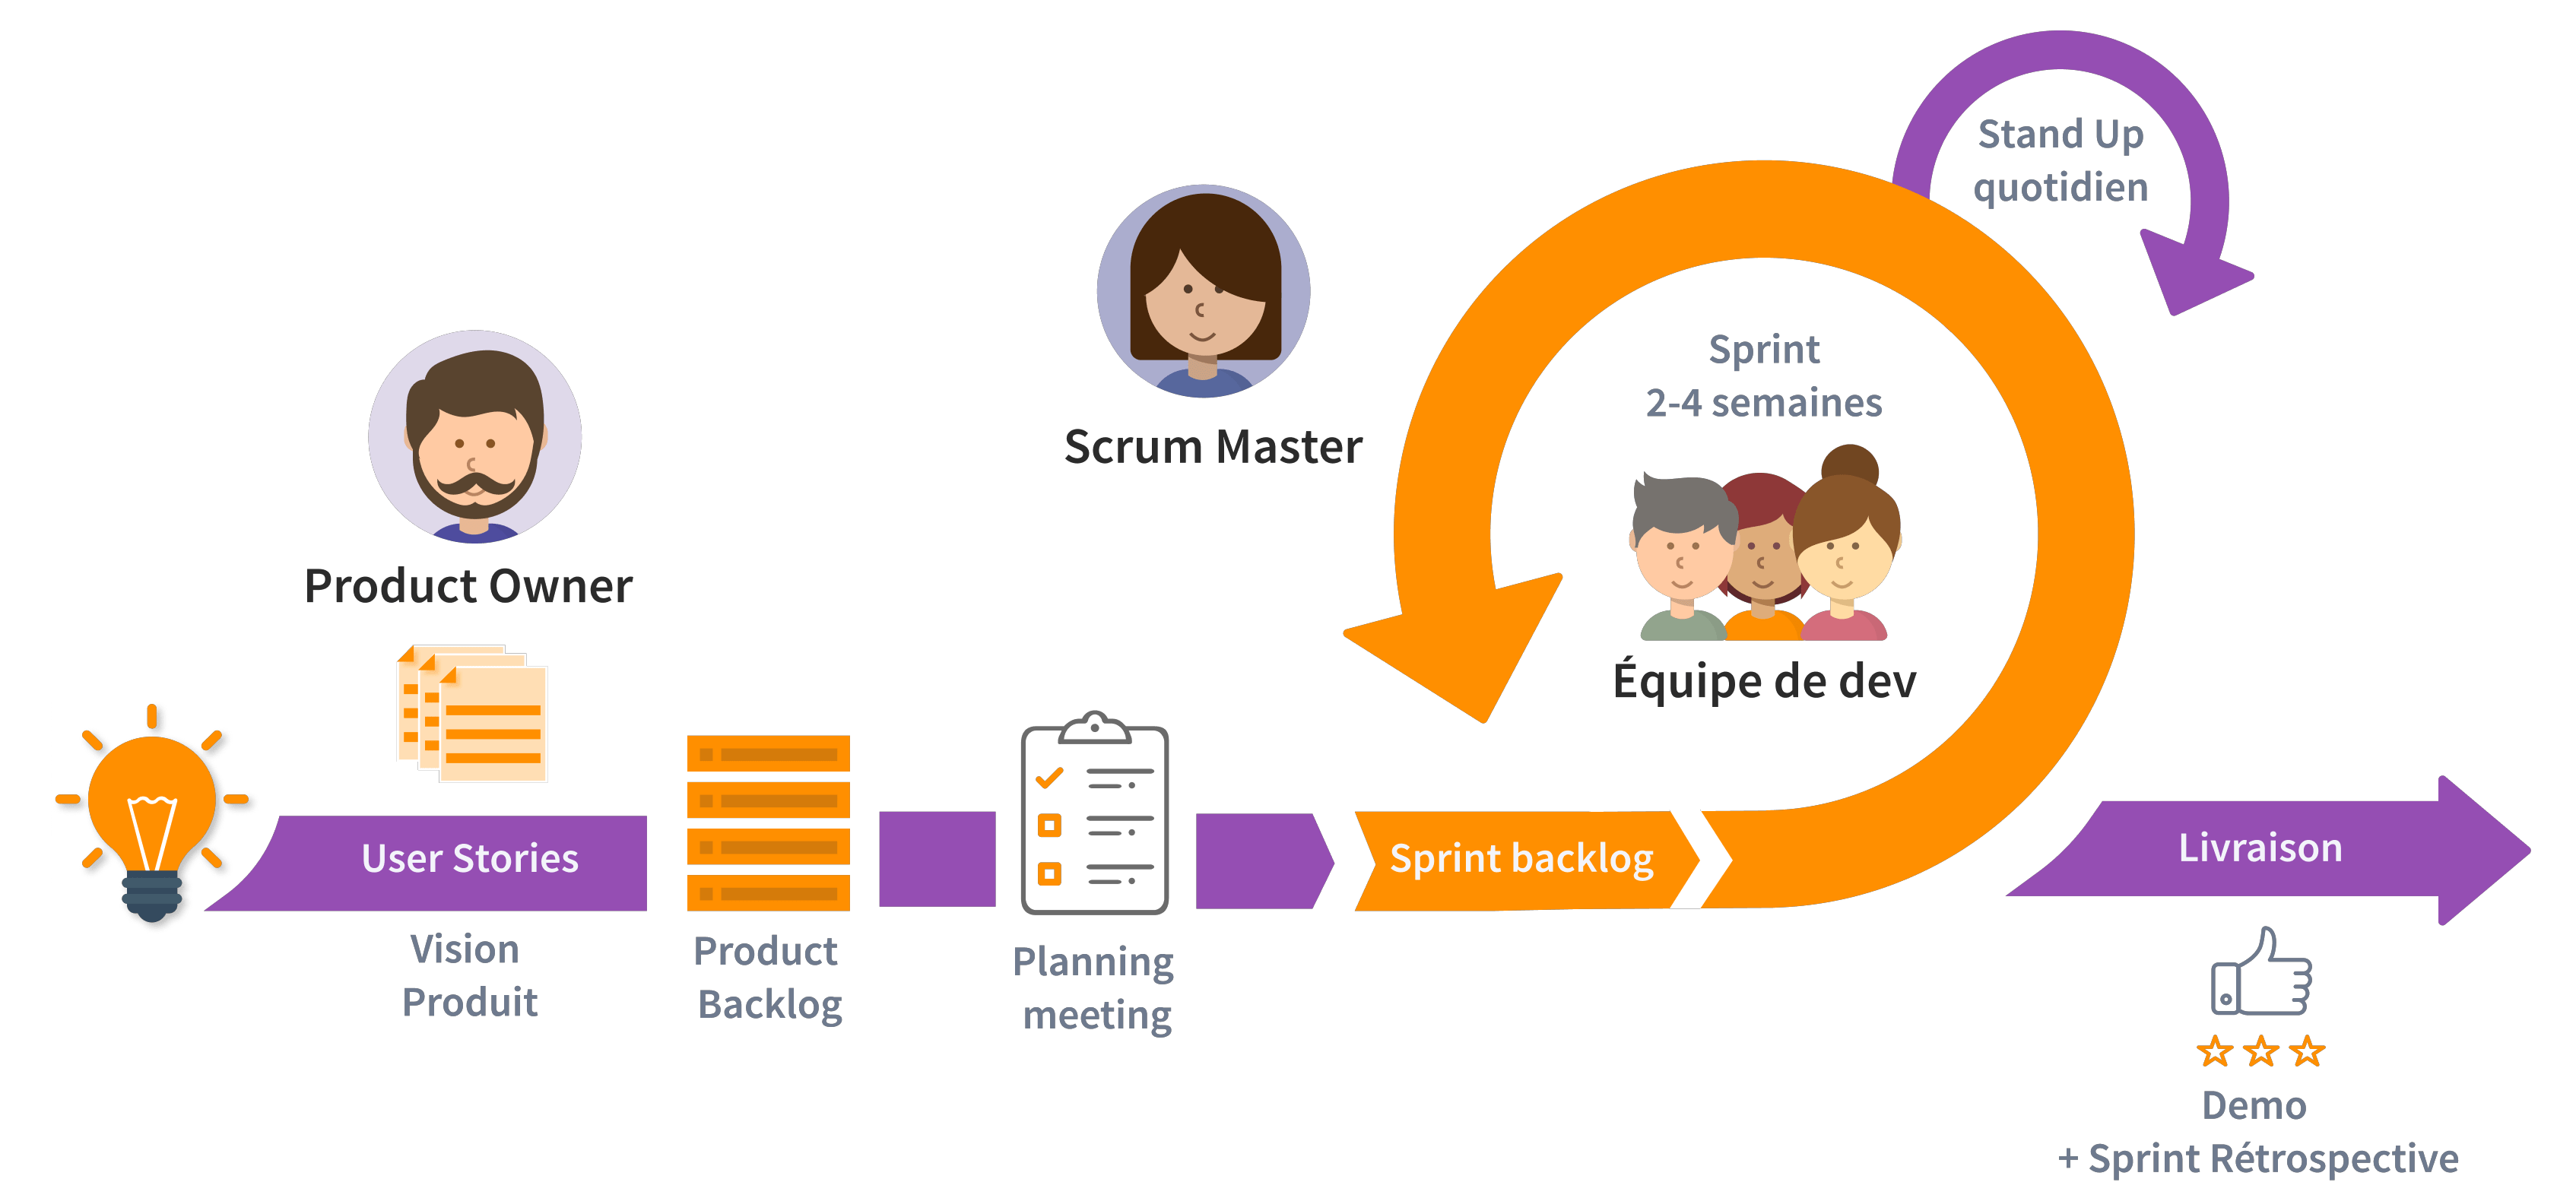
\includegraphics[height=7cm]{agile-Scrum-sprint-workflow-schema-FR.png}}
    \end{center}
    %légende de l'image
    \caption{Processus de méthode Scrum}
\end{figure}

\subsection{\Large Méthode choisir }
\texttt{}\\[0.1cm]

\textsf{\fontfamily{qtm}\selectfont\scalefont{1.3}
Pour la réalisation de notre projet nous avons opté pour la méthodologie agile SCRUM car elle
améliorer la flexibilité de projet et réduit le temps de livraison de produits complet au client.En
effet , la plupart des projets réalisés dans l’entreprise appliquent cette méthodologie.}\\[0.2cm]

\section{\LARGE    Conclusion}
\texttt{}\\[0.3cm]
\textsf{\fontfamily{qtm}\selectfont\scalefont{1.3} Dans ce chapitre nous avons présenté la société d’accueil, la problématique et la méthodologie de développement.
    Dans le prochain chapitre, nous allons faire une étude de l’existant à travers une comparaison des solutions sur le marché afin de proposer notre solution. 
}



%Voici une liste :
%\begin{itemize}
%\item item 1;
%\item item 2;
%\item item 3;
%\item item 4.
%\end{itemize}

%Comment :
%\footnotemark\\

%Detail :
%citation référencé dans le document "bibliographie.bib" inclus à la fin du document

%\footnotetext
